%!TEX root = main.tex
\chapter*{Vorbemerkungen}

\section*{Quellen}

Viele der rein mathematischen Bemerkungen, Aussagen und Beispiele sind Abgeleitet aus \cite{merziger2024repetitorium} und \cite{gollmann2017mathematik}. Im Literaturverzeichnis finden sich selbstverständlich andere zitierte Arbeiten.

\section*{Errata}

Bezüglich etwaigen Fehlern bitte einen \textbf{neuen \emph{issue}} auf github zu eröffnen: \href{https://github.com/hrtlacek/matheFuerTonmeisterinnen/issues}{hier}. Größere Kommentare, Zweifel an Richtigkeit, Feedback etc, sehr gerne auch direkt per mail: \\
\texttt{ptrk.lechner@gmail.com}.

Da ich per email benachrichtigt werde wenn ein \emph{neuer} issue angelegt wird und wir so Überblick behalten wer als erstes den Fehler entdeckt hat, ist dies der bei weitem bevorzugte Weg einen Fehgler zu melden! So sind alle sofort informiert, man kann sehen wenn ein Fehler schon bekannt ist etc.

Sehr gerne können Fehler, Korrekturen und Ergänzungen auch selbst geändert werden und ein \emph{pull request} gemacht werden.

\section*{Hinweise zur Lektüre}

Am Ende dieses Dokuments befinden sich einige praktische Tabellen:
\begin{itemize}
\item Ein Python cheat-sheet, Abschnitt \ref{sec:pythonCheat}
\item Eine Tabelle des Griechischen Alphabets, Abschnitt \ref{sec:greekAlph}
\item Eine kleine Formelsammlung, Abschnitt \ref{sec:formelsam}
\item Nicht zuletzt ein Glossar/Index, Abbildungs- und Literaturverzeichnis etc.
\end{itemize} 

Dieses Dokument benutzt unter anderem folgende Konventionen um verschiedenen Hervorhebungen zu erzielen. 
\important{Besonders Wichtiges und Definitionen}
\example{Durchgerechnete Beispiele}
\praxis{Praxisbezug in der Audiotechnik}

\subsection*{Soundbeispiele}

Soundbeispiele sind in der Programmiersprache \texttt{FAUST} erstellt. Durch click auf das Lautsprecher Symbol sollte sich ein Browser öffnen in dem der entsprechende Klang in Echtzeit berechnet wird. Manche der Beispiele bieten Interaktionsmöglichkeit durch diverse Slider etc. Hier ein Beispiel:

\faust{Sinus, 150 Hz}{https://faustide.grame.fr/?autorun=1&voices=0&name=example&inline=aW1wb3J0KCJzdGRmYXVzdC5saWIiKTsKYW1wID0gaHNsaWRlcigiQW1wbGl0dWRlIiwgMC4yNSwgMCwgMSwgMC4wMDEpOnNpLnNtb287CnByb2Nlc3MgPSAob3Mub3NjKDE1MCkgKiBhbXApIDw6XyxfOw\%3D\%3D}

\emph{Zum Teil scheint es notwendig zu sein noch auf der großen 'RUN' Button links oben zu clicken.}

\begin{figure}[h!]
	\centering
	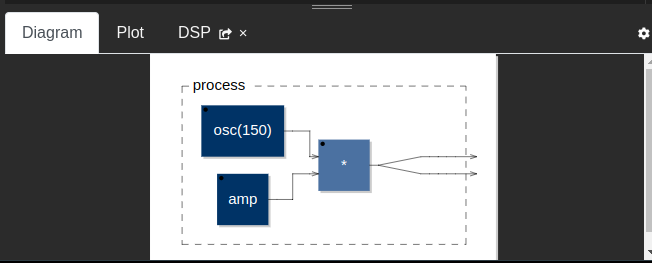
\includegraphics[width=0.8 \textwidth]{img/faust_diag.png}
	\caption{Block Diagramm in \texttt{FAUST}}
	\label{fig:faustBlock}
\end{figure}

Geneigten LeserInnen sei besonders empfohlen auch auf den 'Diagramm' button zu clicken um ein Blockdiagramm zu sehen dass dem Code/dem jeweiligen Konzept Entspricht.

Es kann nicht garantiert werden dass dieses Online-Service ständig online ist und die Details der Programmiersprache \texttt{FAUST} sind \textbf{nicht} Teil des Kurses.

\section*{Contributors}
Hier finden sich hoffentlich bald Menschen die diesen Text gelesen haben und Verbesserungsvorschläge gemacht haben.
\begin{itemize}
	\item Youjin Kim, Fehlerkorrektur in Aufgabe 1.6.
	\item Alexander Simeonov \& Valentin De Ridder, Fehlerkorrektur in Aufgabe 1.6.
	\item Alexander Simeonov, Fehlerkorrektur in Polynom p. 34.
	\item Adrian Fritsche, Fehlerkorrektur in Umformung von $e^{i\pi}=-1$ in Lösung, Kapitel 3, Aufgabe 3, b).
	\item George Sioros, Hinweis, dass es wichtig wäre die Nachteile von \texttt{\%pylab} zu besprechen. Kapitel \ref{cha:funktionen_polynome_python}.
\end{itemize}

% \section*{General TODOs}
% \begin{itemize}
% 	% \item indexing
% 	\item proof reading..
% 	% \item Page numbers
% 	% \item scheinbar wird derzeit teilweise Text 'verschluckt'. zb linearfaktorzerlegung.
% \end{itemize}
